\section{Overhead Evaluation}

This section presents the evaluation of the XCPU3 infrastructure from the
perspective of quicker deployment of a large number of small jobs while giving
clean interfaces and abstractions.

We have performed our evaluations on a Blue Gene setup with 512 nodes.  This
setup is visually presented in a figure \ref{fig:hare}.  We run hosted Inferno
on all the compute nodes, IO nodes and the controller node.  The user interacts 
with the XCPU3 instance on the controller node for job submission.

\begin{figure}[h]
  \begin{center}
    \leavevmode
      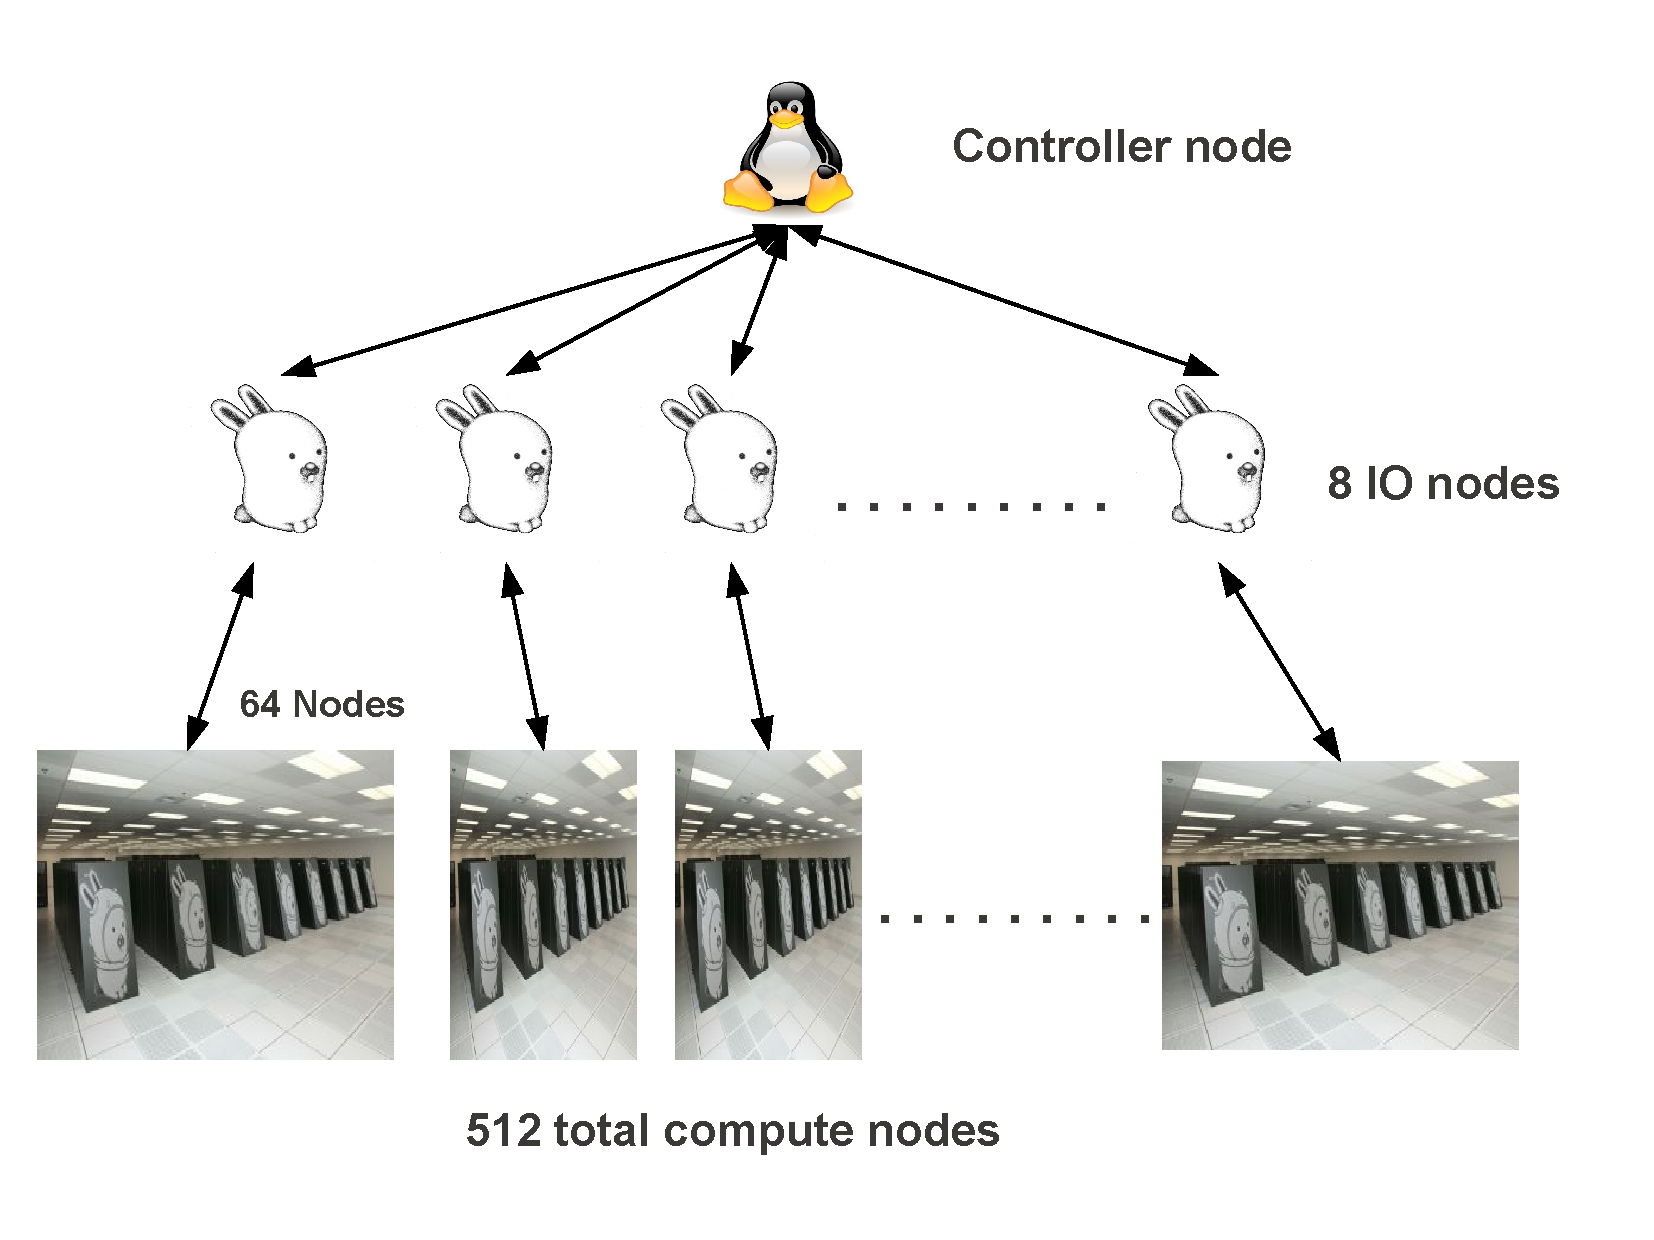
\includegraphics[height=0.2\textheight,width=0.4\textwidth]
		{./img/EvaluationSetup}
    \caption{Setup for evaluation}
    \label{fig:hare}
  \end{center}
\end{figure}

\subsection{Execution}

Our first objective is to show how quickly we can do deployment and execution
of a large number of small applications. We have avoided using larger
applications as the bigger runtimes of larger applications tend to amortize the
overhead in the deployment of the application.  We have used the \texttt{date}
command as the application for deployment.  This is a small application and does
not need any external inputs and produces small output. Each deployment involves
session creation, reservation, execution, output aggregation and termination
of the session.  We deployed varying numbers of execution of this application on
the cluster of 512 nodes.  The number of requested executions increased
exponentially from 1 to 2048 executions.

\begin{figure}[h]
  \begin{center}
    \leavevmode
      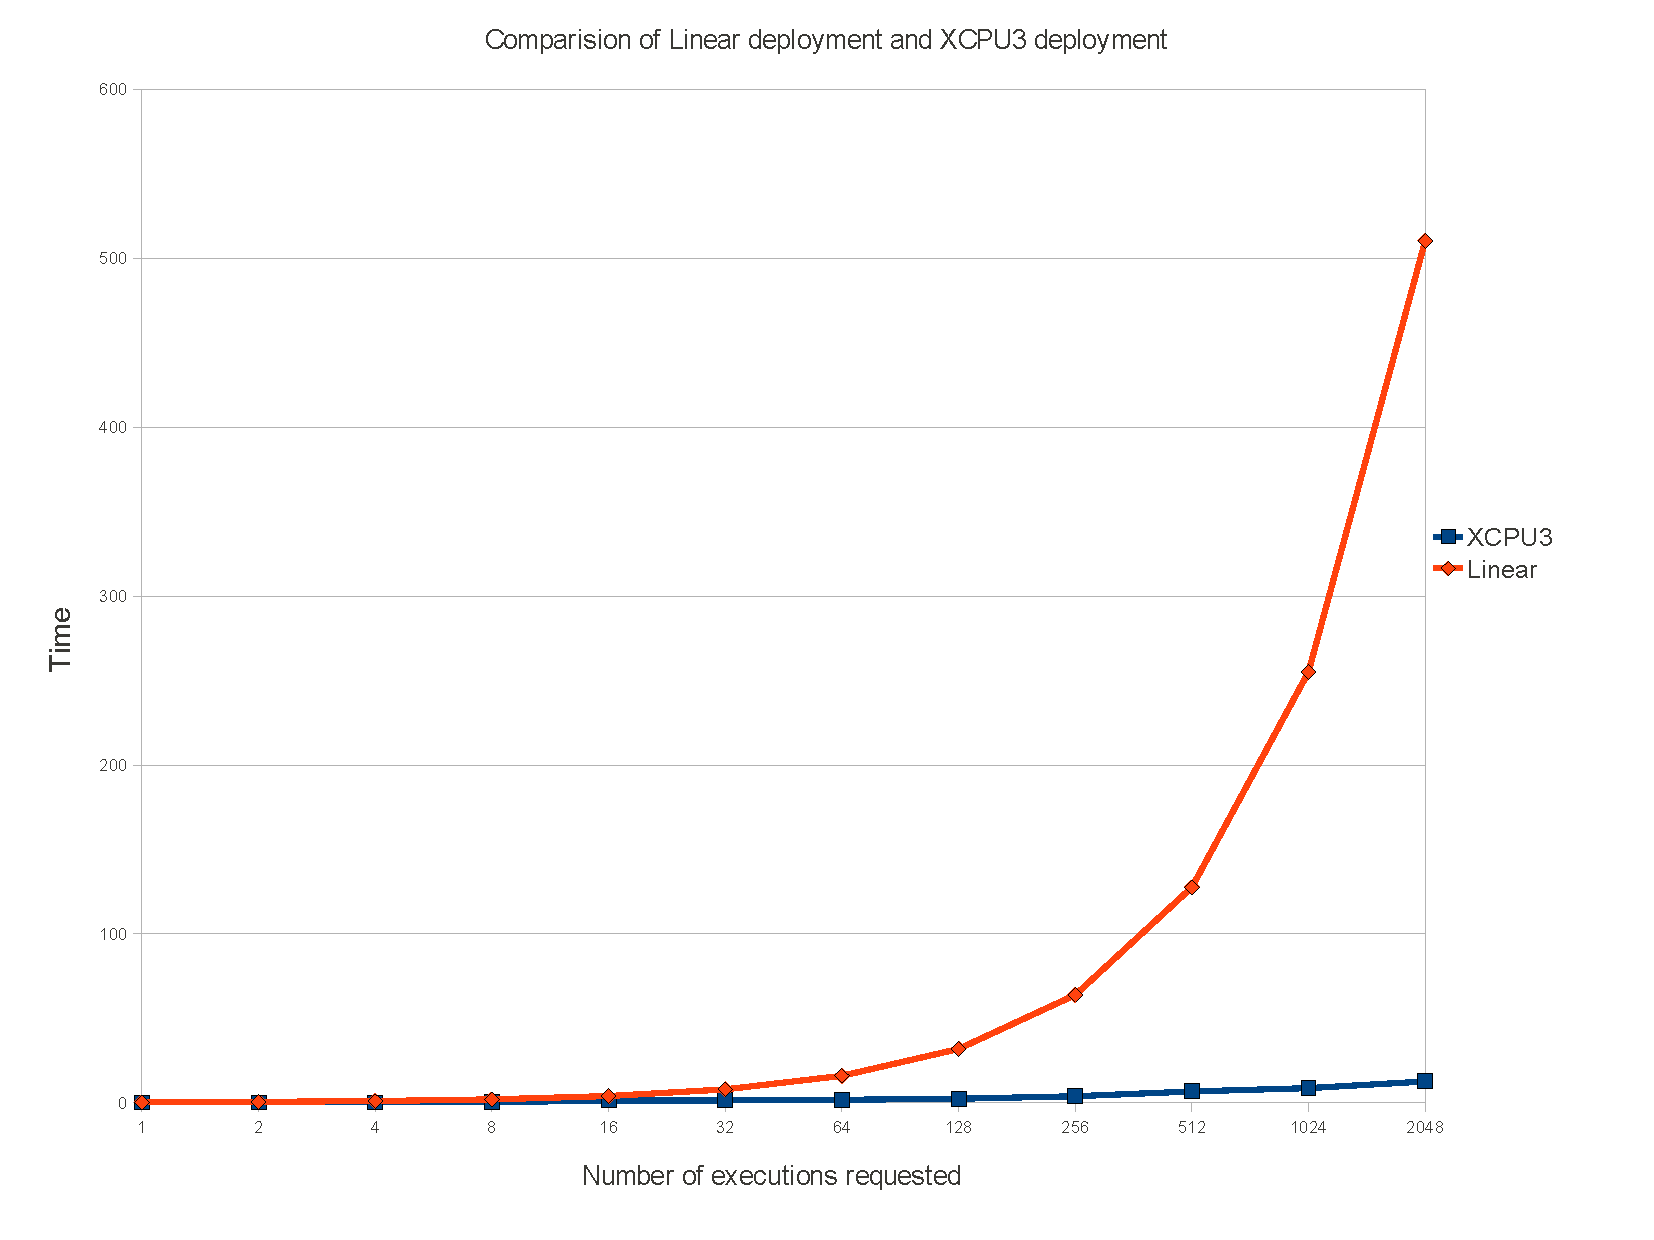
\includegraphics[height=0.2\textheight,width=0.5\textwidth]
		{./img/linear}
    \caption{Comparison if XCPU3 with sequential deployment}
    \label{fig:sequential}
  \end{center}
\end{figure}

Figure \ref{fig:sequential} gives an initial perspective of how XCPU3 performs
relative to sequential performance.  This graph plots the total time taken by
XCPU3 and the hypothetical time it may take for performing the same amount of
work on one machine.  This graph shows that the XCPU3 is successfully able to
exploit the parallelism for deploying the jobs quickly. The XCPU3 deploys 2048
jobs in 12.66 seconds whereas sequential execution would take upto 510 seconds.
In the graph, the line showing sequential scaling looks exponential, but that is
because number of requested executions increase exponentially.

\subsection{Communication}

This section aims to further analyze the performance of XCPU3.  Again we are 
concentrating on similar deployment.  We have recorded the time taken by each
of the following stages in the deployment on the XCPU3 infrastructure.

\begin{enumerate}
\item Reservation: Create a new session, and request the reservation by writing
\texttt{res n} into the session \texttt{[ctl]} file.  Here \textbf{n} varies
from 1 to 2048 representing the number of executions requested. 

\item Execution: Request the execution by writing \texttt{exec date} into the
session \texttt{[ctl]} file.

\item Aggregation: Collect the output generated by all the executions by reading
the session \texttt{[stdio]} file.

\item Termination: Closing all the files and terminating the session.

\item Housekeeping: Additional time taken before, between and after above steps.
\end{enumerate}
Every deployment starts with the creation of the session followed by the
reservation, execution, aggregation and then ending with termination of the
session.  We have taken the average value over multiple runs for our analysis.

\begin{figure}[h]
  \begin{center}
    \leavevmode
      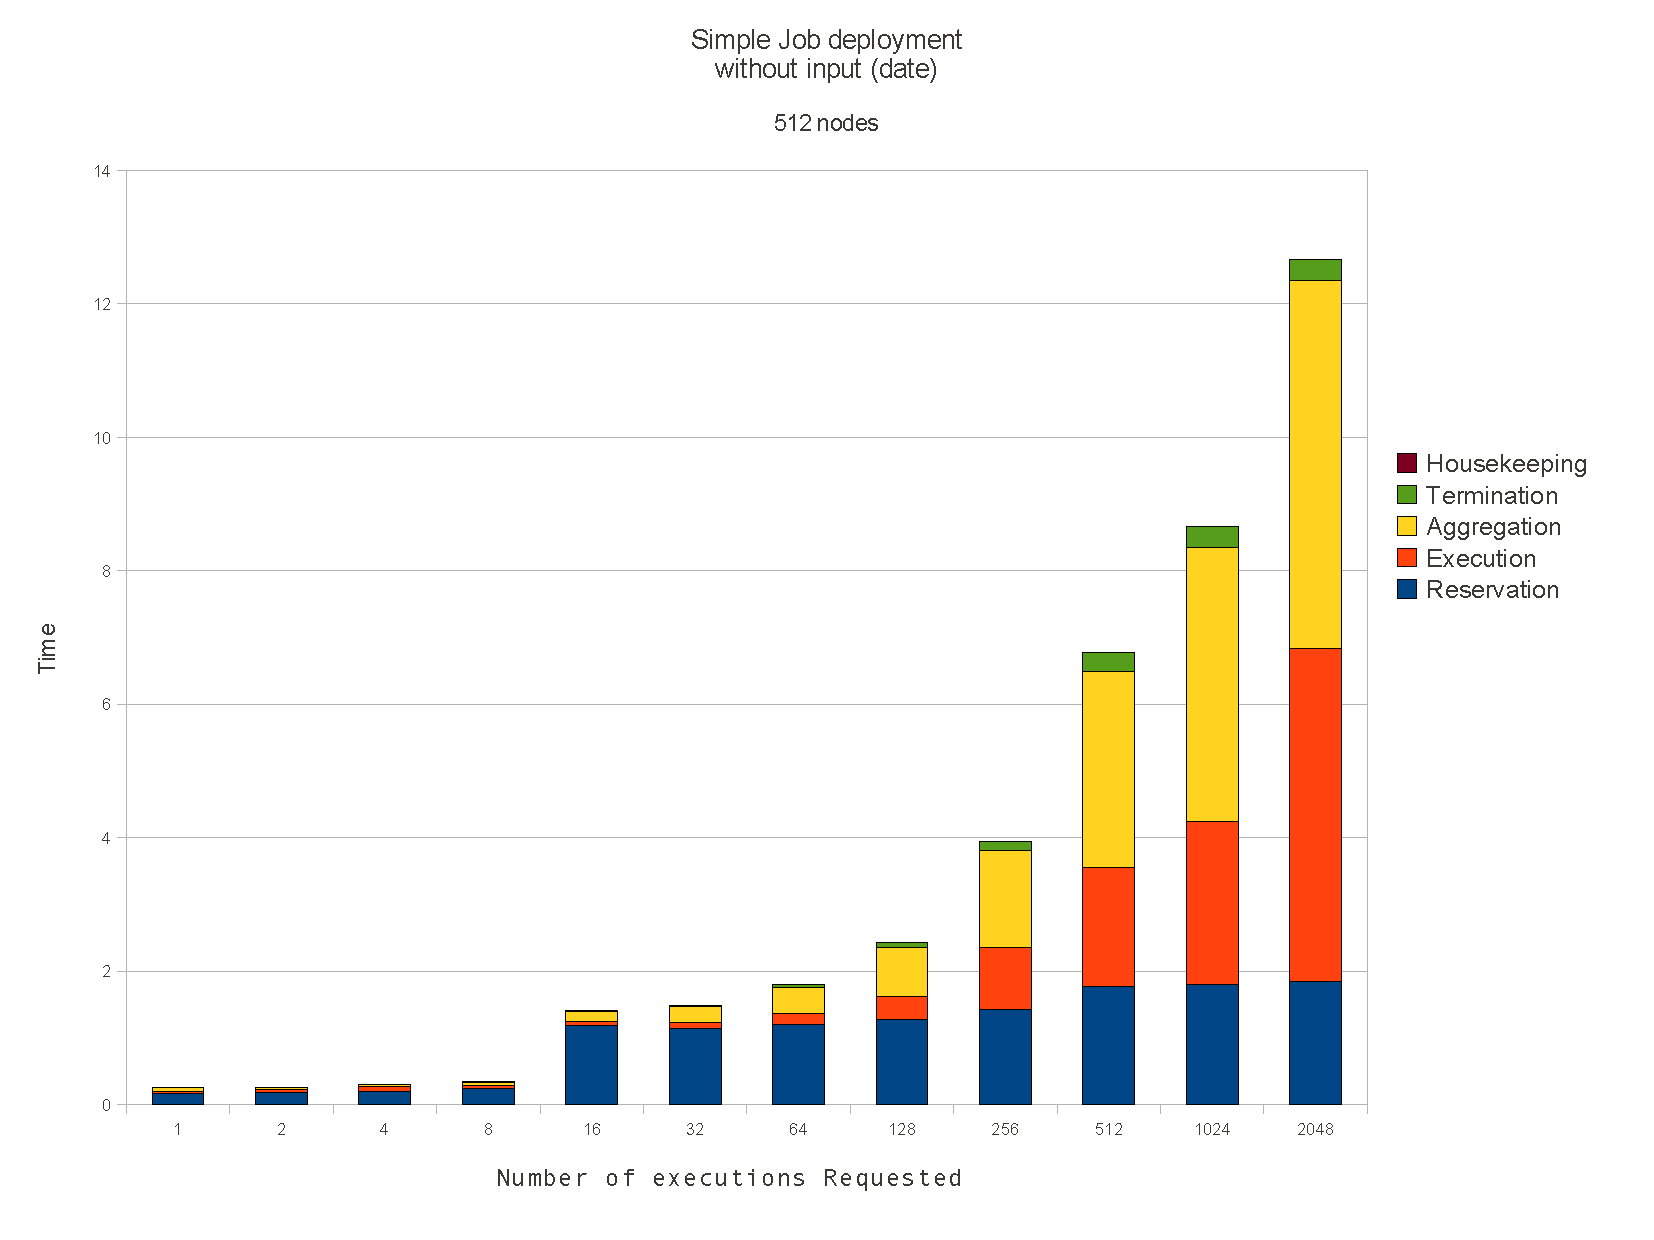
\includegraphics[height=0.2\textheight,width=0.5\textwidth]
		{./img/date_graph}
    \caption{Deployment without input}
    \label{fig:date_graph}
  \end{center}
\end{figure}

Figure \ref{fig:date_graph} presents the results of deployment of the date
command in the form of graph.  This graph presents the breakup time for various
stages of the deployment using the XCPU3 infrastructure.

From this graph we can observe that the session termination and the housekeeping
overheads are negligible compared to the time taken by reservation, execution
and aggregation.  So, we can ignore these two overheads in our future
evaluations.  For jobs of up to 128 deployments, the reservation time dominates
everything else.  But for larger numbers of deployment execution and
aggregation time increases rapidly while reservation time remains relatively
constant. This shows that reservation time is not directly dependent on
the number of deployments, whereas execution and aggregation time are directly
proportional to the number of deployments.

Now, let us try to analyze why reservation time is independent of the number of
deployments.  The reservation process involves traversing the underlying
topology tree of nodes till the reservation requirements are satisfied.  All the
children on the same level are traversed parallelly at the same time.  This way,
each level is traversed in the constant time, independent of number of nodes in
that level.  Another aspect of the reservation mechanism which helps here is
that the amount of data written and read from the \texttt{[ctl]} file and the
amount of data exchanged between nodes for communicating reservation request is
fixed in size and independent of the number of deployments requested.  With
these two properties, the reservation time becomes directly proportional to the
depth of the tree and not with the number of nodes.

We can observe the above relation in figure \ref{fig:date_graph}. The 
reservation time remains relatively constant for deployment requests from 1 to
8.  Then it sharply increases between 8 to 16 and remains almost constant for
all the requests between 16 to 2048.  This can be attributed to underlying
cluster topology. Figure \ref{fig:hare} shows the presence of the 8 IO nodes
in the first level. This enables satisfying the requests which are smaller
than 8 executions. For larger requests, one more level needs to be traversed
in the topology, introducing delays.  The time taken for reservation remains
almost constant between 16 and 2048 executions as all these reservation
requests essentially traverses the same depth.  We can conclude from these
observations that \textit{the time taken for the reservation is directly
proportional to the depth of the tree}.

Now let us discuss, why the same property is not exhibited by execution time or
aggregation time. We have discussed in the implementation chapter that all
read and write requests are performed in parallel between all the nodes in the
same level.  But the amount of data exchanged for aggregation and execution is
not constant.  This data is directly proportional to the number of nodes
involved.  With the increase in the number of requested deployments, the
amount of data to be exchanged also increases, leading to larger aggregation
time. The execution time is also similarly affected as all compute nodes will
try to fetch the binary of the executable from the initiating node leading to
the copy of the data. These observations lead us to to conclusion that
\textit{the time taken for the execution and aggregation is directly
proportional to the number of deployments requested}.

Our next evaluation involve the deployment of an executable \texttt{wc} which
needs input. This command counts the number of lines, words and characters in
the input file.  This is an interesting case for our infrastructure as this
deployment involves the distribution of inputs to all the sessions.  This
introduces a new stage in the deployment process in addition to the 5 stages we
described in the above section.  This stage will be the \textbf{input} stage and
involves distributing the input data to all the sessions which are responsible
for execution.  By default XCPU3 will broadcast the input to all the compute
nodes, but we have plans to introduce filters in the PUSH shell which can
partition the input given to the compute  nodes. 

Figure \ref{fig:wc_graph} presents the results of evaluations involving the
distribution of the input.


\begin{figure}[h]
  \begin{center}
    \leavevmode
      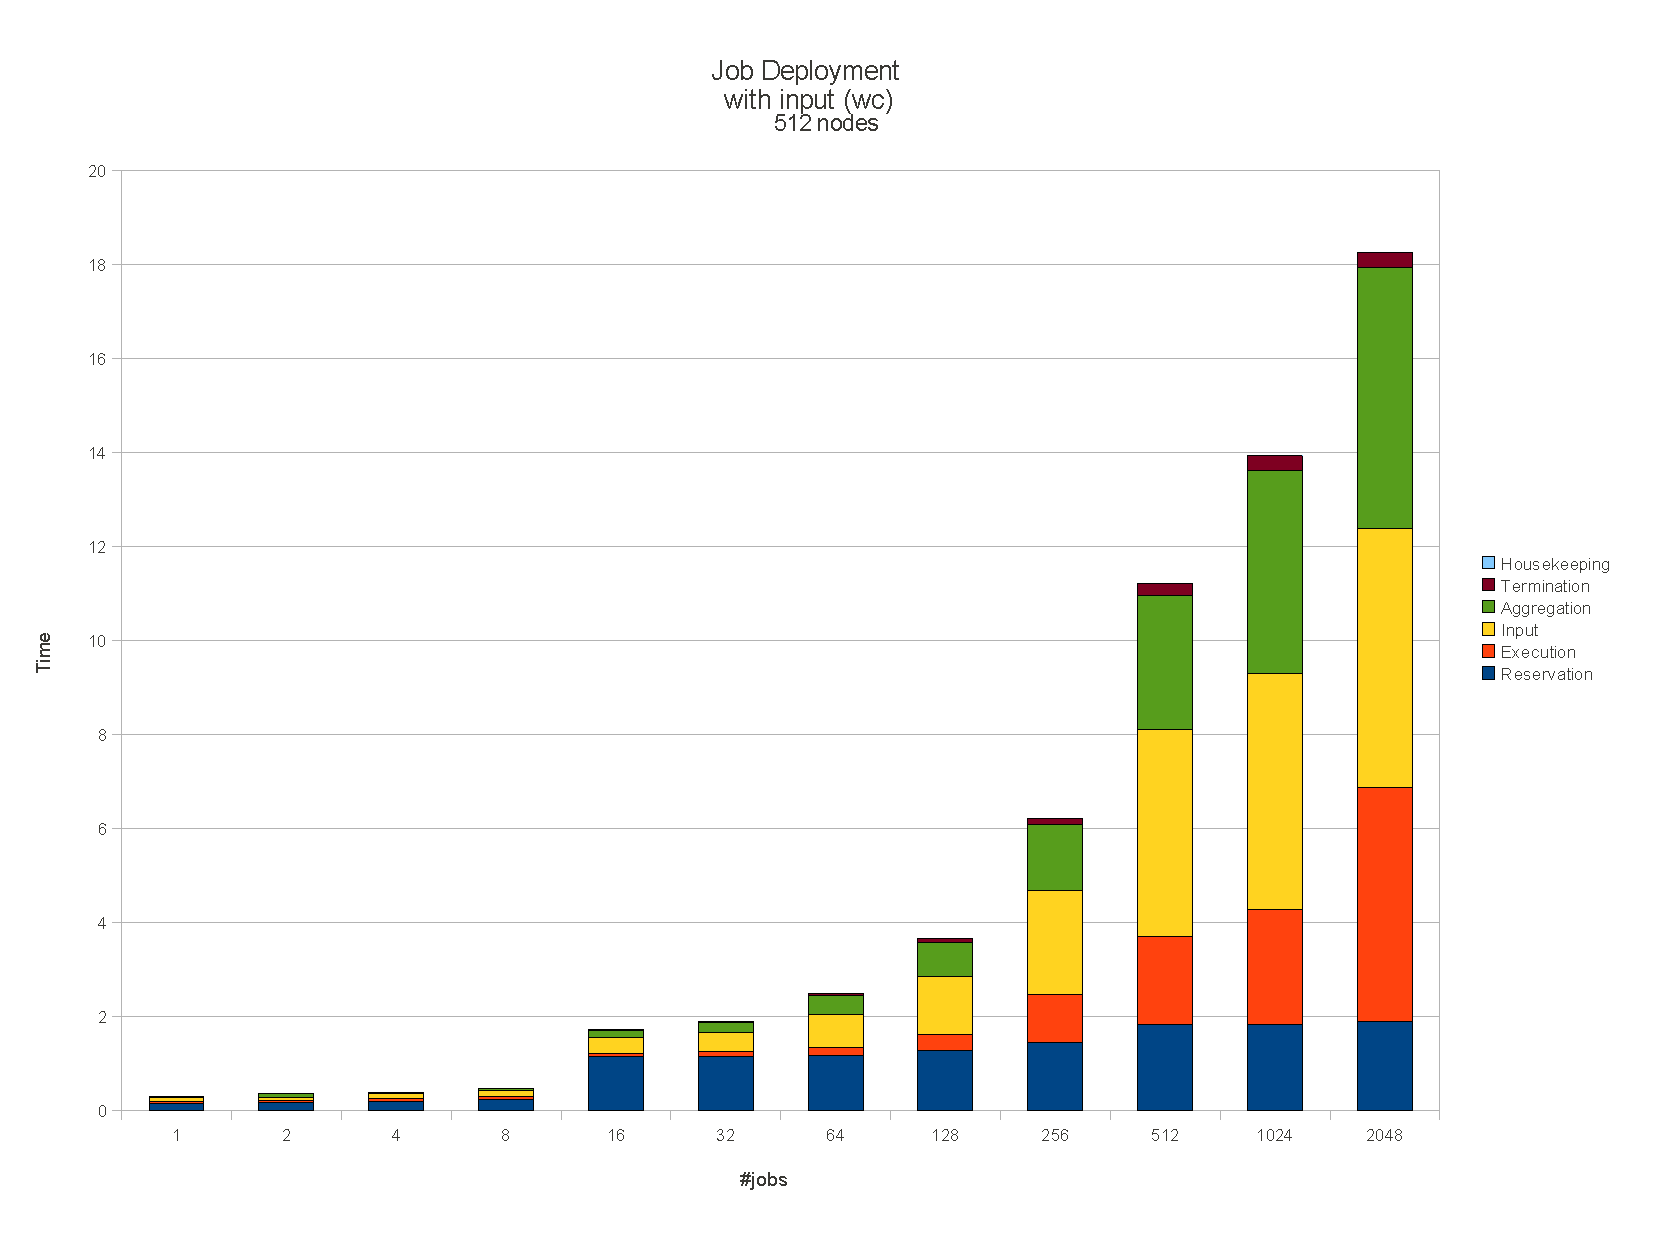
\includegraphics[height=0.2\textheight,width=0.5\textwidth]
		{./img/wc_graph}
    \caption{Deployment with input}
    \label{fig:wc_graph}
  \end{center}
\end{figure}

These results enforce our observations that reservation time is directly
proportional to the the depth of the tree whereas aggregation and execution time
are directly proportional to the number of deployments requested.  In addition
to these observations, we can also observe that the input time exhibits 
behavior similar to the execution and aggregation time.  This observation can be
attributed to the fact that input distribution implementation is similar
to the output aggregation implementation.  And also the amount of data to be
exchanged for input distribution depend on the number of deployments requested
as this data needs to reach all sessions responsible for execution.  This
increases the amount of data to be exchanged with any increase in the number of
the deployments requested.  We can conclude with this observation that
\textit{the input time is directly proportional to the number of deployments
requested}

\subsection{Dataflow}
The evaluations presented in this chapter helps us in understanding how fast
XCPU3 can deploy small jobs and aggregate the results produced by them.  Now
let us relate how these observations can justify our claims about dataflow
applications. Typical deployments of the dataflow applications are similar to
the above experiments as it involves starting up a large number of small jobs.
But the similarity is over at this point. Dataflow deployment does not always
involve the input distribution and output aggregation stages.  These deployments
work by feeding the output of one computation as input for other computation. 
At the end of the computation, a user needs to read the output of only selected
compute sessions which does not need any aggregation.  What we can conclude from
the above description is that XCPU3 performs really well in the stages like
reservation which are important for dataflow deployments.  The stages like input
distributions are output aggregation where XCPU3 is relatively slow are not
needed by dataflow deployments.  This makes XCPU3 ideal for rapid deployment of
dataflow workloads.

Unfortunately we do not have concrete measurements and evaluations to back our
predictions.  XCPU3 is one of the piece in the envisioned solution for problem
of efficient and easy deployment of large-scale dataflow applications.   We are
still working on the integration of userspace applications like
PUSH\cite{PODC:Push} with XCPU3 which will further simplify the dataflow
deployment.

XCPU3 is an infrastructure which provides the needed flexibility, speed and 
ease of use for dataflow workloads.  This chapter demonstrates the speed that
can be achieved.  It is difficult to measure the properties like \textit{ease of
use} and \textit{flexibility} but the examples presented in the filesystem
interface chapter should give some insights of all the possibilities opened up
by the XCPU3.

